\lab{Algorithm}{Change of Basis}{Change of Basis}
\label{lab:ChangeBasis}

\objective{Understand how to change the basis of a set of points.}

\section*{Basis}

A basis for a vector space is a set of vectors such that every vector in the space can be expressed uniquely as a linear combination of the basis vectors. In this lab we will take the coordinates in 2-d space and do various affine transformations. For all these exercises we will use the points
\begin{lstlisting}
A=np.array([-1.5,-1.,-.5,0.,.5,1.,1.5,.75,-.75],[0.,-1.,-2.,-2.,-2.,-1.,0.,2.,2.])
\end{lstlisting}
Let A be the matrix of points and M is the matrix that will perform the affine transformation (TODO: find out the correct word). So $M*A$ will be the set of points in the new basis. 

\section*{stretch}
To stretch a set of points, M will be a diagonal matrix where the value in each position is the stretch in that direction.

\begin{figure}[H]
%\begin{center}
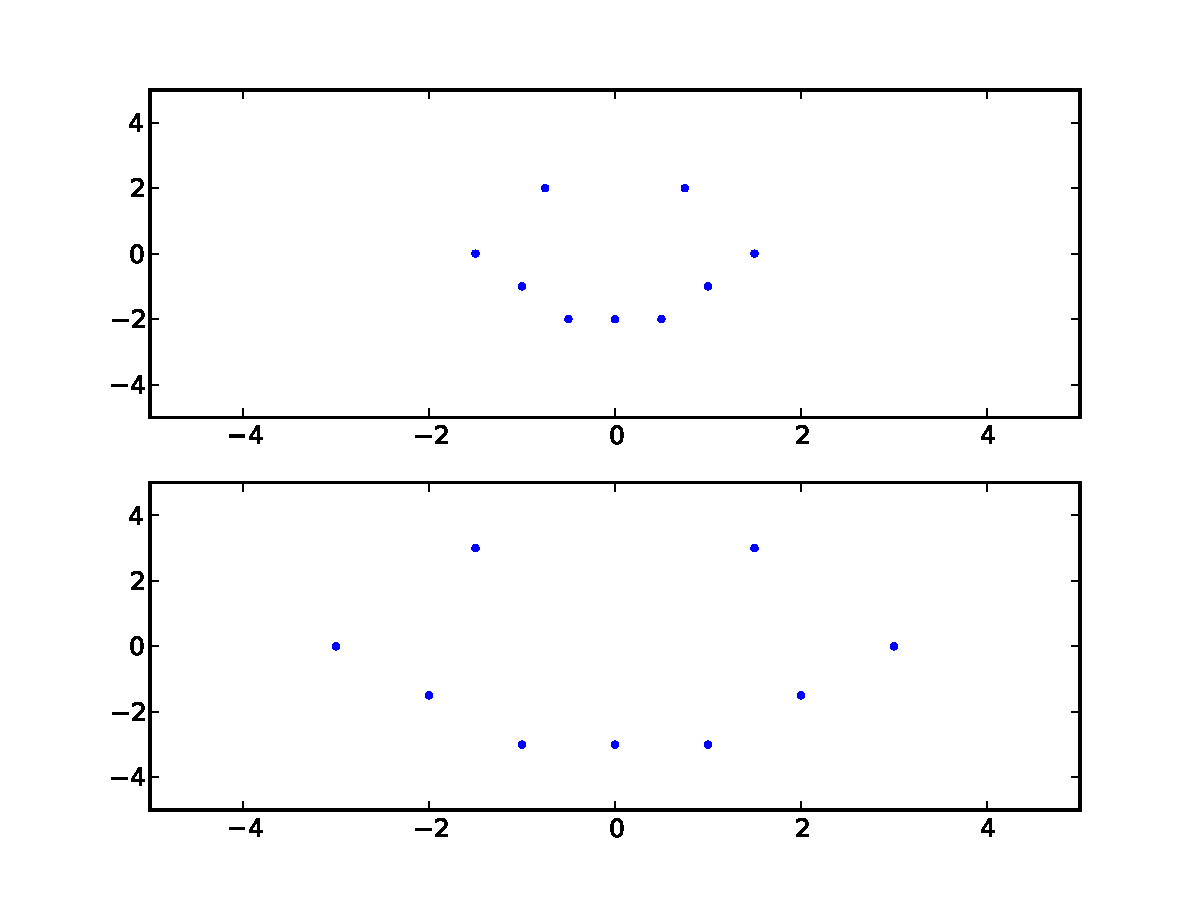
\includegraphics[scale = .5]{strench.pdf}
\caption{An example of a stretch. The top image is the original and the bottom is the modified image. The streach was 2 in the x direction and 1.5 in the y direction.}
%\end{center}
\end{figure}

\begin{problem}
Write a function that will accepts a matrix of points and how much to stretch them in each direction. Have the function plot the transformed points.
\end{problem}

\section*{Rotation}
To do a rotation clockwise a set of points in angle $\theta$ (where $\theta$ is in radians) let
\[
M = \begin{pmatrix}
\cos(\theta) & -\sin(\theta) \\
\sin(\theta) & \cos(\theta) 
\end{pmatrix}
\]

\begin{figure}[H]
%\begin{center}
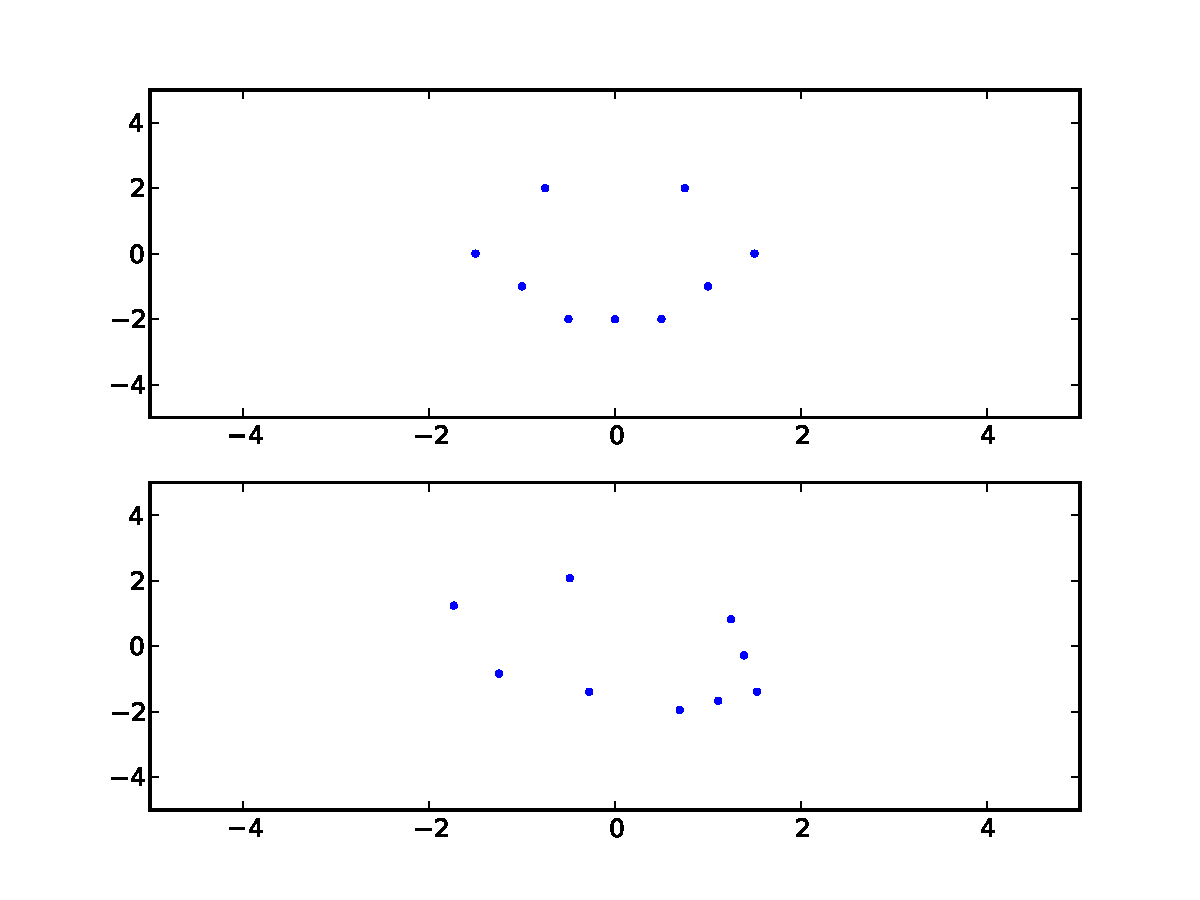
\includegraphics[scale = .5]{rotate.pdf}
\caption{An example of a rotate. The top image is the original and the bottom is the modified image. The rotation angle was $\frac{3\pi}{16}$.}
%\end{center}
\end{figure}

\begin{problem}
Write a function that will accepts a matrix of points and how many radians to rotate the points. Have the function plot the transformed points.
\end{problem}

\section*{Shift}
Let L be vector that represents shift that you add to A. In order to shift a set of points, you add to the row how much you would like it to shift it in that direction. So to shift the set of points up by 2, $L=[0,2]$. You can use array broadcasting to do this.

\begin{figure}[H]
%\begin{center}
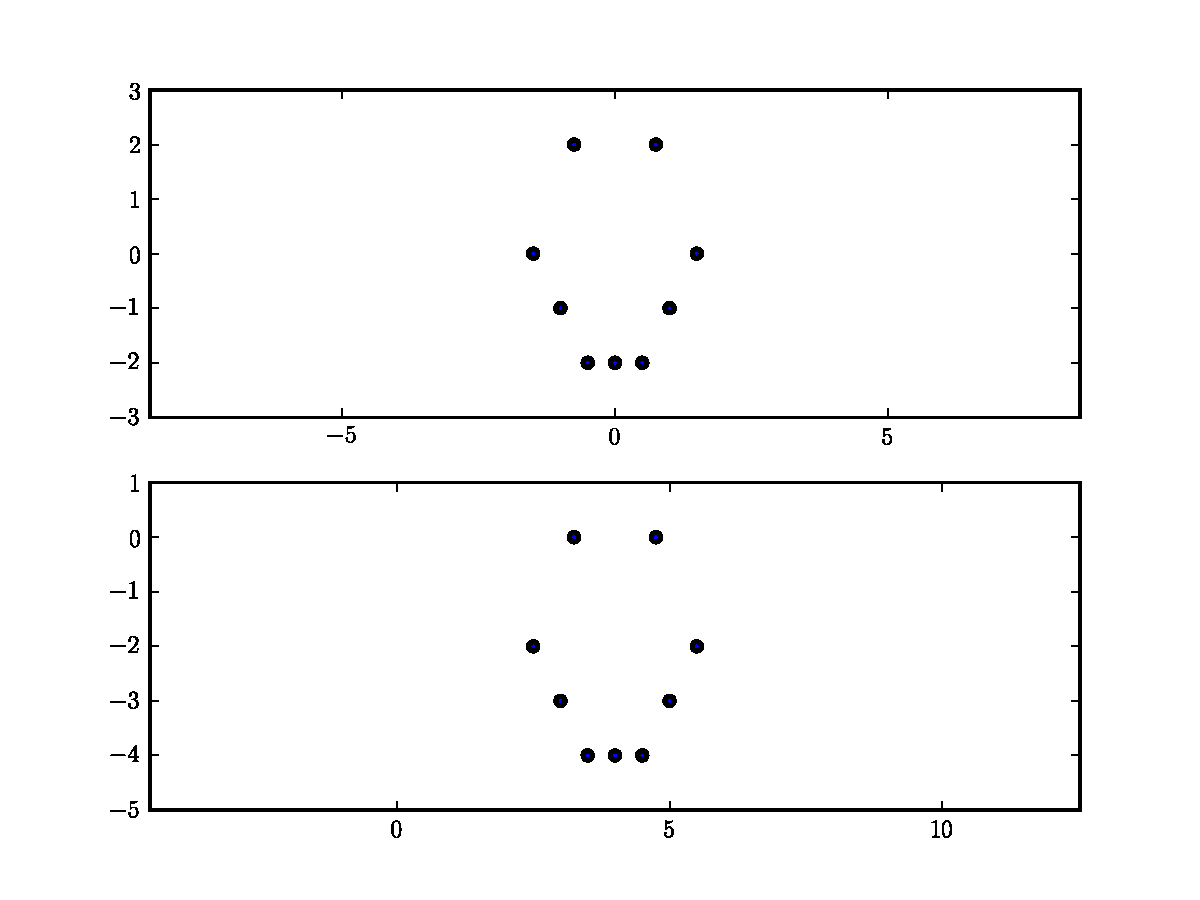
\includegraphics[scale = .5]{shift.pdf}
\caption{An example of a shift. The top image is the original and the bottom is the modified image. The shift was 2 in the x direction and 1 in the y direction.}
%\end{center}
\end{figure}

\begin{problem}
Write a function that will accepts a matrix of points and how much to shift them in each direction. Have the function plot the transformed points.
\end{problem}

\section*{Combination}
Say you have points in a rotated basis and you want to stretch them along that basis. You left multiply the strech matrix $S$ by the rotation matrix $R$. So $R*S*A$ will stretch the points in the rotation in R. 

\begin{figure}[H]
%\begin{center}
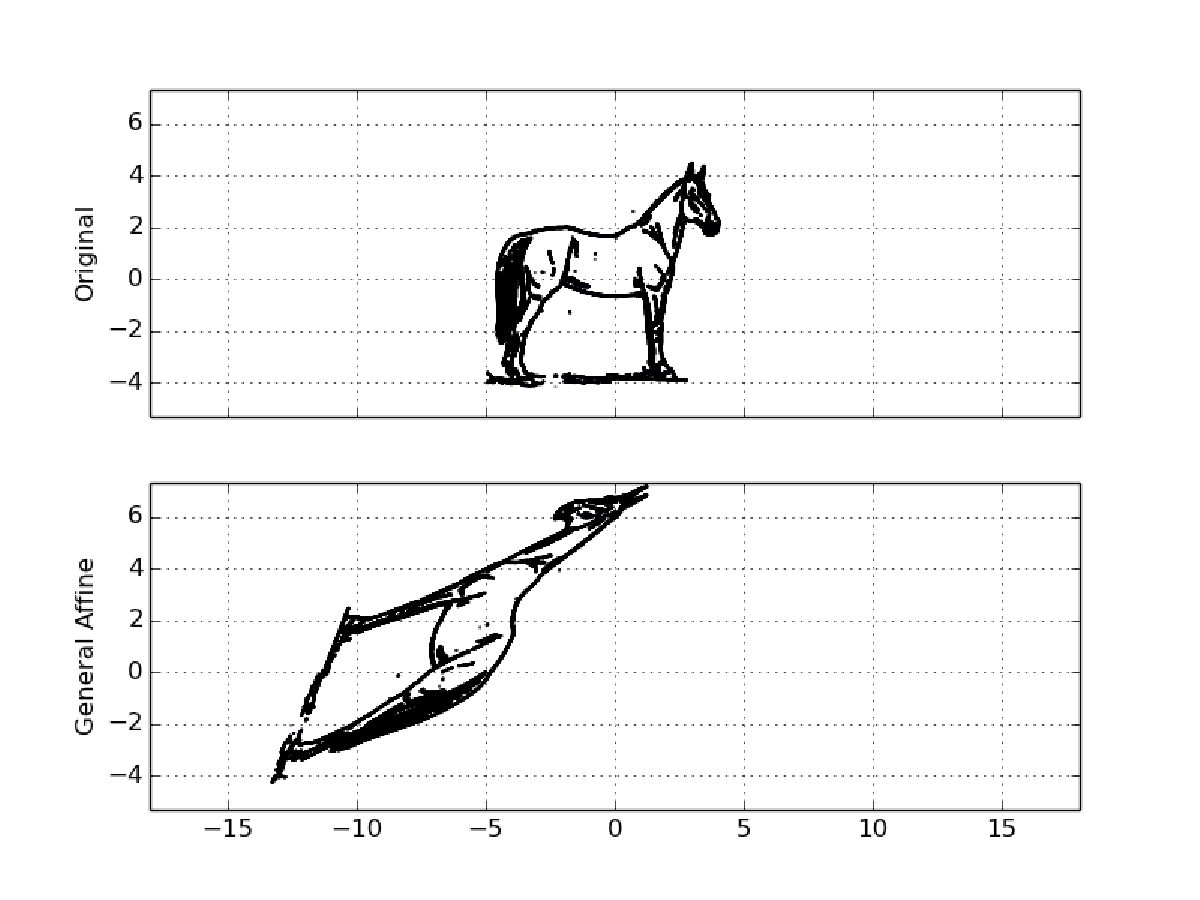
\includegraphics[scale = .5]{combo.pdf}
\caption{A combination. The stretch was 2 in each direction. The rotation angle was $\frac{3\pi}{4}$. The shift was 1 in the x direction and -2 in the y direction.}
%\end{center}
\end{figure}

\begin{problem}
Write a function that will accepts a matrix of points and stretch, rotate and shift them.
\end{problem}

\section*{Images}

An Image is a 3d array where the first two dimensions are the location and the 3rd dimension is the RGB content. To apply the above transformations one would need to moved the position of the RGB arrays to match where the new transformation would have them. Stretching is done by
 interpolation.

\begin{figure}[H]
%\begin{center}

\includegraphics[scale = 2.0]{dream.png}
\caption{The original image}
%\end{center}
\end{figure}

\begin{figure}[H]
%\begin{center}
\includegraphics[scale = .5]{rotateimg.pdf}
\caption{Rotated at an angle of $\frac{\pi}{4}$}
%\end{center}
\end{figure}

\begin{problem}
Write a function that will accepts an image and how many radians to rotate the image. The function will rotate the image around the center of the image and then show the rotated image. HINTS: Make an array of ones that is $1.5$ times greater than the max of the height and width of the original image. Change the x,y coordinates in the original image so the center is $(0,0)$. Rotate the image and then center the image. You might need to use for loops. Allow your test cases to be small images.
\end{problem}


